\PassOptionsToPackage{dvipsnames}{xcolor}
\documentclass[14pt]{beamer}
\usepackage{beamerthemesplit}
\usepackage{amsmath,amssymb,amsthm, epsfig, pdflscape, MnSymbol, hyperref}
\theoremstyle{plain}
\newtheorem*{thm}{Theorem}
\newtheorem*{pro}{Proposition}
\newtheorem*{lem}{Lemma}
\newtheorem*{cor}{Corollary}
\newtheorem*{con}{Conjecture}
\newtheorem*{que}{Question}
\newtheorem*{cla}{Claim}
\theoremstyle{definition}
\newtheorem*{defi}{Definition}
\newtheorem*{ack}{Acknowledgements}
\theoremstyle{remark}
\newtheorem*{rem}{Remark}
\newtheorem*{rems}{Remarks}
\newtheorem*{eg}{Example}
\newtheorem*{exs}{Examples}
\newtheorem*{ex}{Exercise}
\mode<presentation>
\setbeamertemplate{background canvas}[vertical shading][bottom=red!10,top=blue!10] 
\usetheme{Warsaw}
\usecolortheme{spruce}
\beamertemplatenavigationsymbolsempty
\usefonttheme[onlysmall]{structurebold}
\setbeamercolor{structure}{fg=NavyBlue}
\setbeamercolor{author in head/foot}{fg=white}
\usepackage{graphicx}


\title{Virtual Reality}
\author{Nick Pietras}
\institute{Franciscan University of Steubenville}
\date{} 



\begin{document}
\begin{frame}
\titlepage
\end{frame}

\begin{frame}{Interest}
\begin{center}
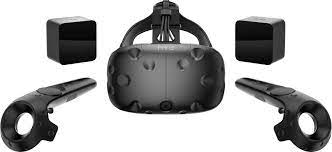
\includegraphics[width=3.4in]{Image HTC_VIVE.jpg}
\end{center}
\tiny{\textbf{Fig. 1.} Buy VIVE Hardware | VIVE European Union. https://www.vive.com/eu/product/vive/. Accessed 13 Apr. 2022.}
\end{frame}

\begin{frame}{Terminology}
Virtual Reality (VR)
\vskip .2in
Augmented Reality (AR)
\vskip .2in
Mixed Reality (MR)
\vskip .2in
Extended Reality (XR)
\end{frame}

\begin{frame}{Virtual Reality}
\begin{center}
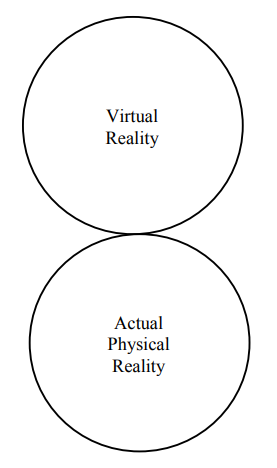
\includegraphics[height=2in]{Image VR1.png} 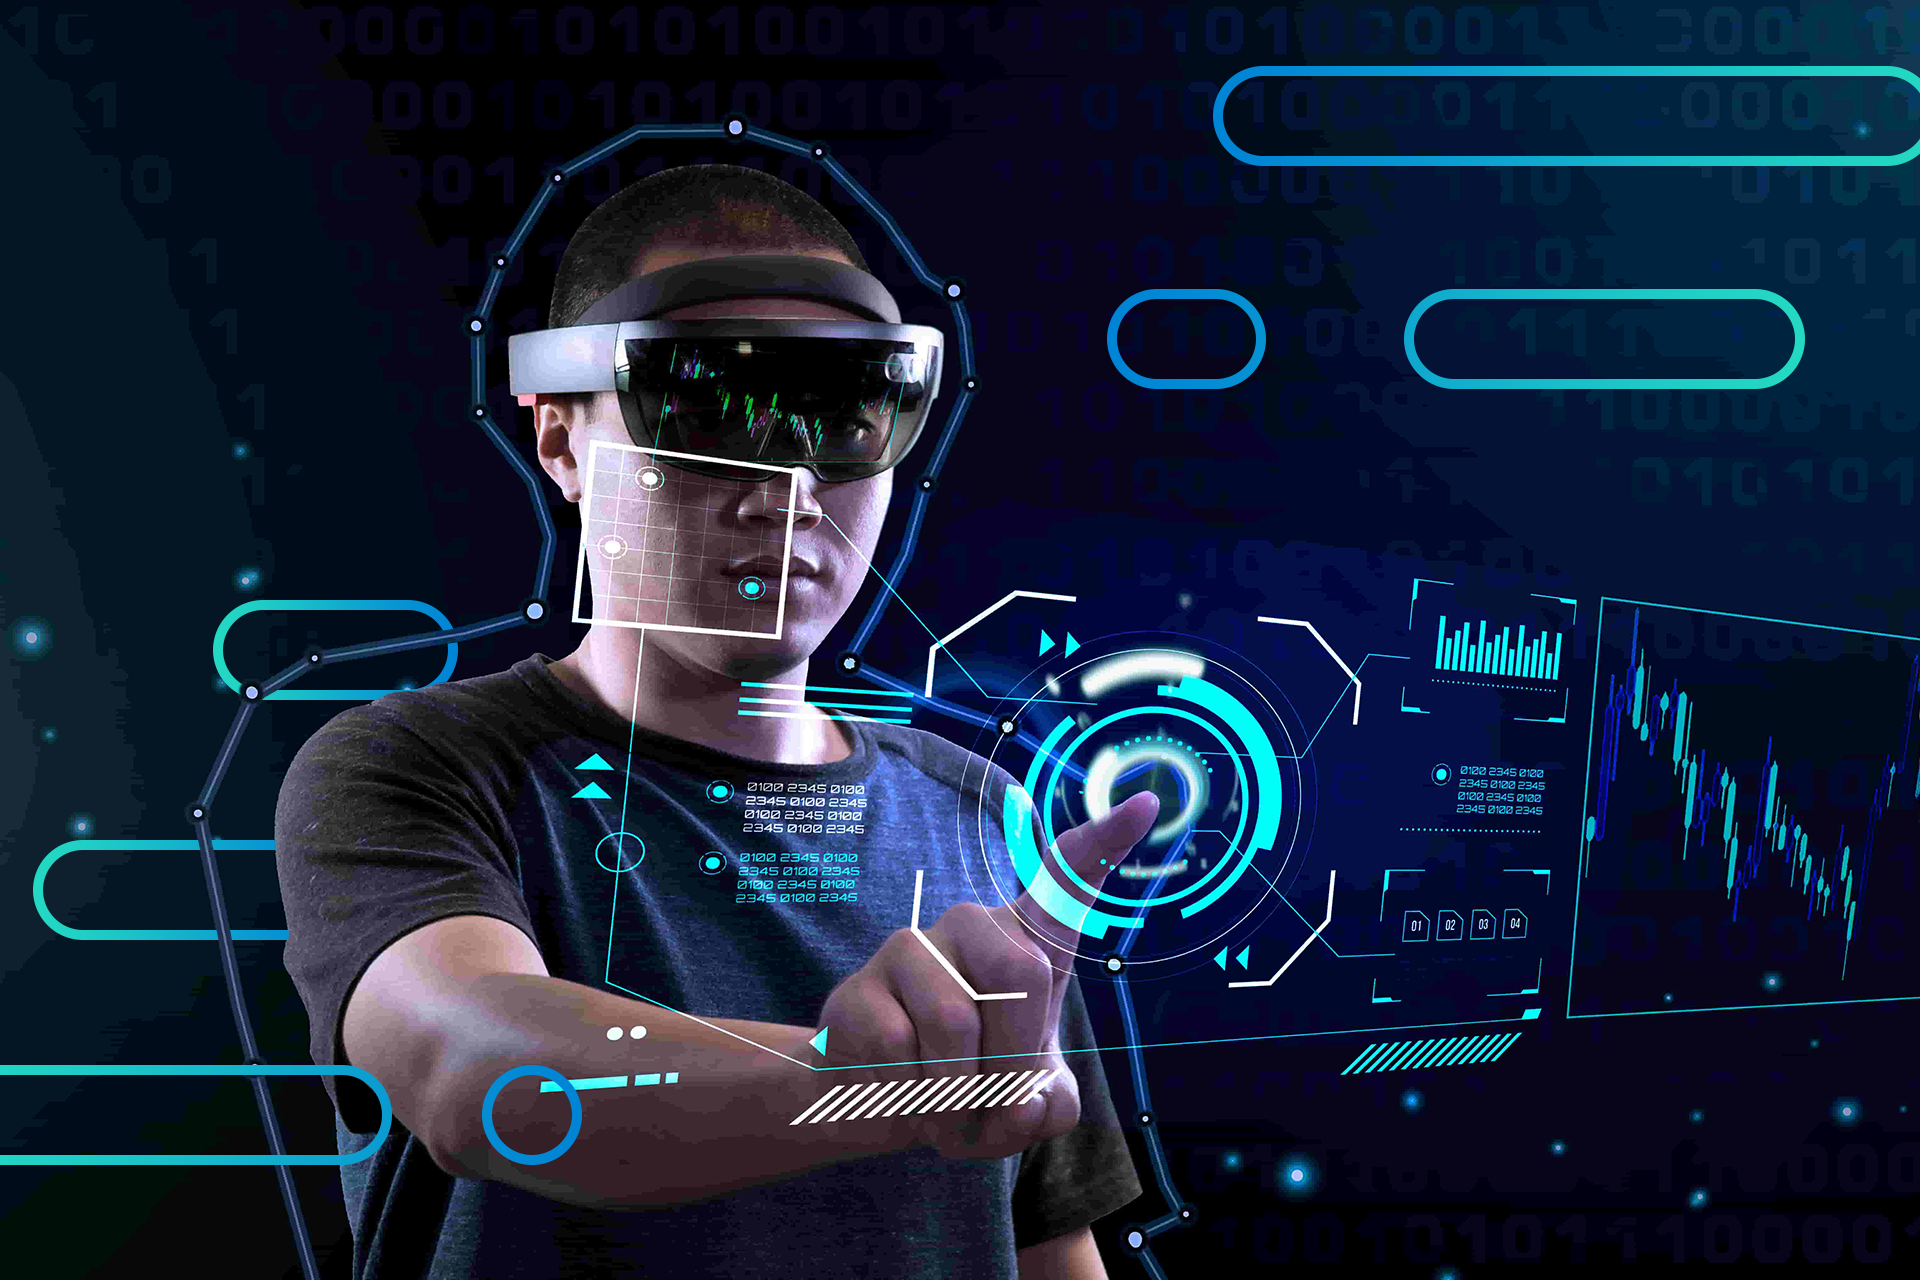
\includegraphics[height=2in]{Image VR2.png}
\end{center}
\tiny{\textbf{Fig. 2. (Left)} Verma, Jitendra Kumar, and Sudip Paul, editors. Advances in Augmented Reality and Virtual Reality. Springer Singapore, 2022. DOI.org (Crossref), https://doi.org/10.1007/978-981-16-7220-0.}
\vskip .1in
\tiny{\textbf{Fig. 3. (Right)} “Virtual Reality, Pros & Cons. A Closer Look at the Future.” Optimum, https://www.optimum.com/articles/internet/the-realities-of-virtual-reality. Accessed 13 Apr. 2022.}
\end{frame}

\begin{frame}{Augmented Reality}
\begin{center}
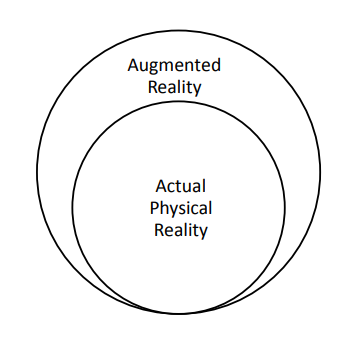
\includegraphics[height=1.6in]{Image AR1.png} 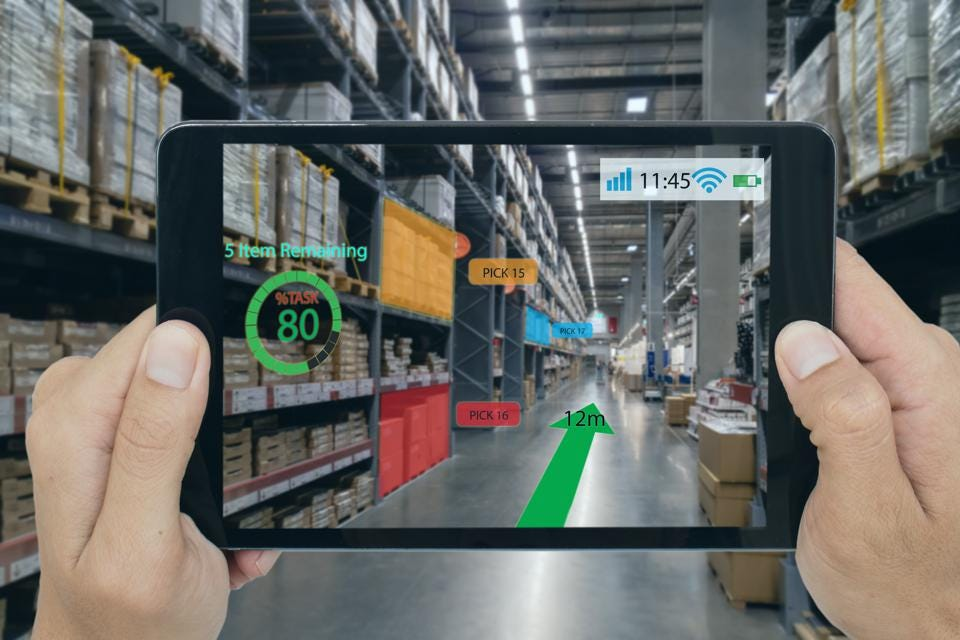
\includegraphics[height=1.6in]{Image AR2.jpg}
\end{center}
\tiny{\textbf{Fig. 4. (Left)} Verma, Jitendra Kumar, and Sudip Paul, editors. Advances in Augmented Reality and Virtual Reality. Springer Singapore, 2022. DOI.org (Crossref), https://doi.org/10.1007/978-981-16-7220-0.}
\vskip .1in
\tiny{\textbf{Fig. 5. (Right)} Council, Young Entrepreneur. “Council Post: Augmented Reality In Business: How AR May Change The Way We Work.” Forbes, https://www.forbes.com/sites/theyec/2019/02/06/augmented-reality-in-business-how-ar-may-change-the-way-we-work/. Accessed 13 Apr. 2022.}
\end{frame}

\begin{frame}{Mixed Reality}
\begin{center}
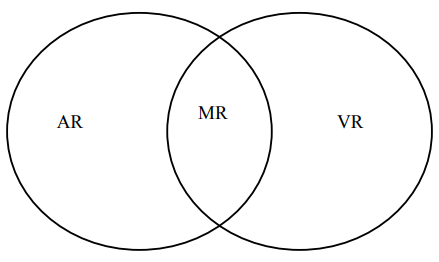
\includegraphics[width=2.2in]{Image MR1.png} 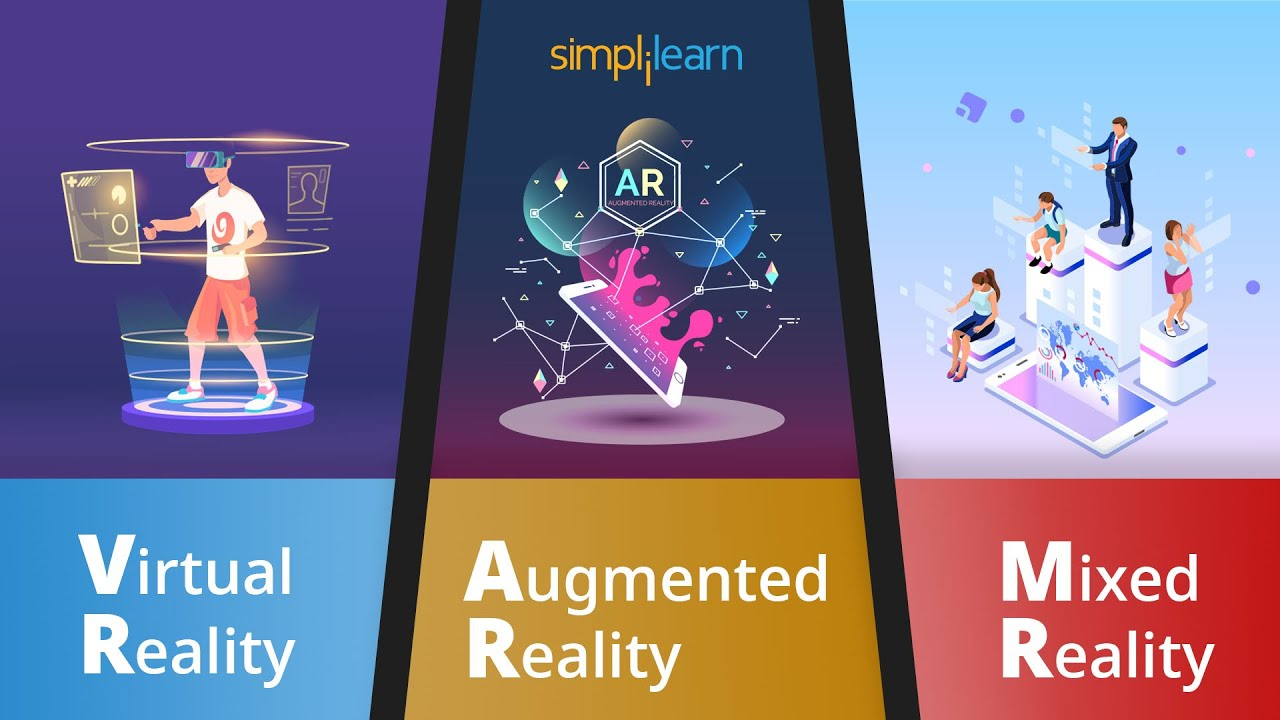
\includegraphics[width=2.2in]{Image MR2.jpg}
\end{center}
\tiny{\textbf{Fig. 6. (Top)} Verma, Jitendra Kumar, and Sudip Paul, editors. Advances in Augmented Reality and Virtual Reality. Springer Singapore, 2022. DOI.org (Crossref), https://doi.org/10.1007/978-981-16-7220-0.}
\vskip .1in
\tiny{\textbf{Fig. 7. (Bottom)} The Rise Of Technology-Augmented Reality(AR), Virtual Reality(VR) And Mixed Reality(MR) |Simplilearn - YouTube. https://www.youtube.com/watch?v=XLP4YTpUpBI. Accessed 13 Apr. 2022.}
\end{frame}

\begin{frame}{Extended Reality}
\begin{center}
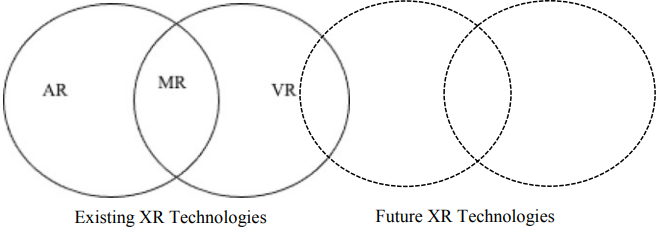
\includegraphics[width=2.4in]{Image XR1.png} 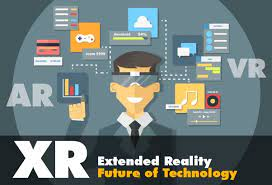
\includegraphics[width=2.4in]{Image XR2.jpg}
\end{center}
\tiny{\textbf{Fig. 8. (Top)} Verma, Jitendra Kumar, and Sudip Paul, editors. Advances in Augmented Reality and Virtual Reality. Springer Singapore, 2022. DOI.org (Crossref), https://doi.org/10.1007/978-981-16-7220-0.}
\vskip .1in
\tiny{\textbf{Fig. 9. (Bottom)} What Is Extended Reality (XR)? – Reality Technologies. https://reality-technologies-europe.com/extended-reality/. Accessed 13 Apr. 2022.}

\end{frame}

\begin{frame}{History of Virtual Reality}
\begin{center}
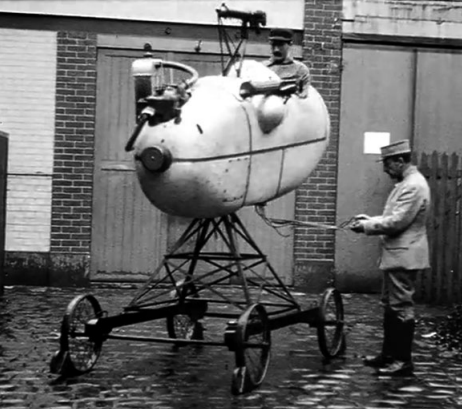
\includegraphics[width=3in]{Image History1.png}
\end{center}
\tiny{\textbf{Fig. 10.} Grasnick, Armin. Basics of Virtual Reality: From the Discovery of Perspective to VR Glasses. Springer Berlin Heidelberg, 2021. DOI.org (Crossref), https://doi.org/10.1007/978-3-662-64201-6.}
\end{frame}

\begin{frame}{History of Virtual Reality}
\begin{center}
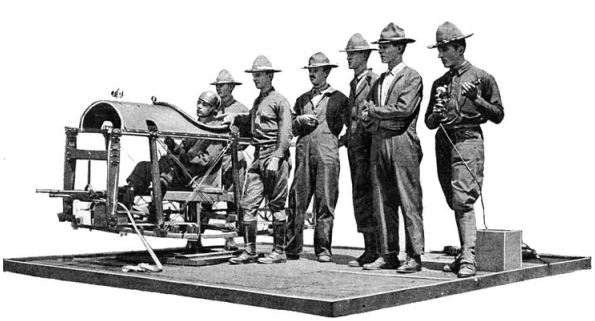
\includegraphics[width=3.8in]{Image History2.png}
\end{center}
\tiny{\textbf{Fig. 11.} Grasnick, Armin. Basics of Virtual Reality: From the Discovery of Perspective to VR Glasses. Springer Berlin Heidelberg, 2021. DOI.org (Crossref), https://doi.org/10.1007/978-3-662-64201-6.}
\end{frame}

\begin{frame}{History of Virtual Reality}
\begin{center}
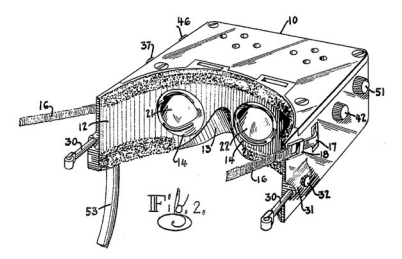
\includegraphics[width=3.6in]{Image Heilig.png}
\end{center}
\tiny{\textbf{Fig. 12.} Six Degrees of Freedom - Wikiwand. https://www.wikiwand.com/en/Six_degrees_of_freedom. Accessed 2 Apr. 2022.}
\end{frame}

\begin{frame}{Six Directions of Freedom}
\begin{center}
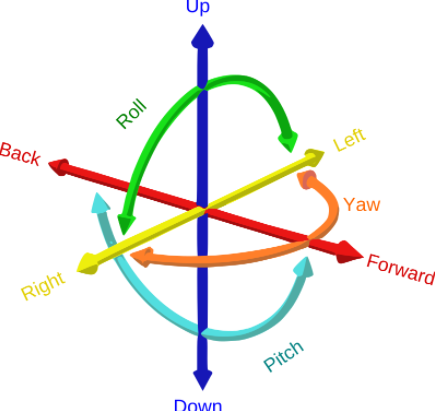
\includegraphics[width=3in]{Image 6DOF.png}
\end{center}
\tiny{\textbf{Fig. 13.} Six Degrees of Freedom - Wikiwand. https://www.wikiwand.com/en/Six_degrees_of_freedom. Accessed 2 Apr. 2022.}
\end{frame}

\begin{frame}{Devices Used for Detecting Motion}
Virtual Reality headsets use three different kinds of machines for detecting motion along the six directions of freedom:
\vskip .2in
\begin{itemize}
    \item Gyroscopes
    \vskip .2in
    \item Accelerometers
    \vskip .2in
    \item Magnetometers
\end{itemize}
\end{frame}

\begin{frame}{Gyroscopes}
\begin{center}
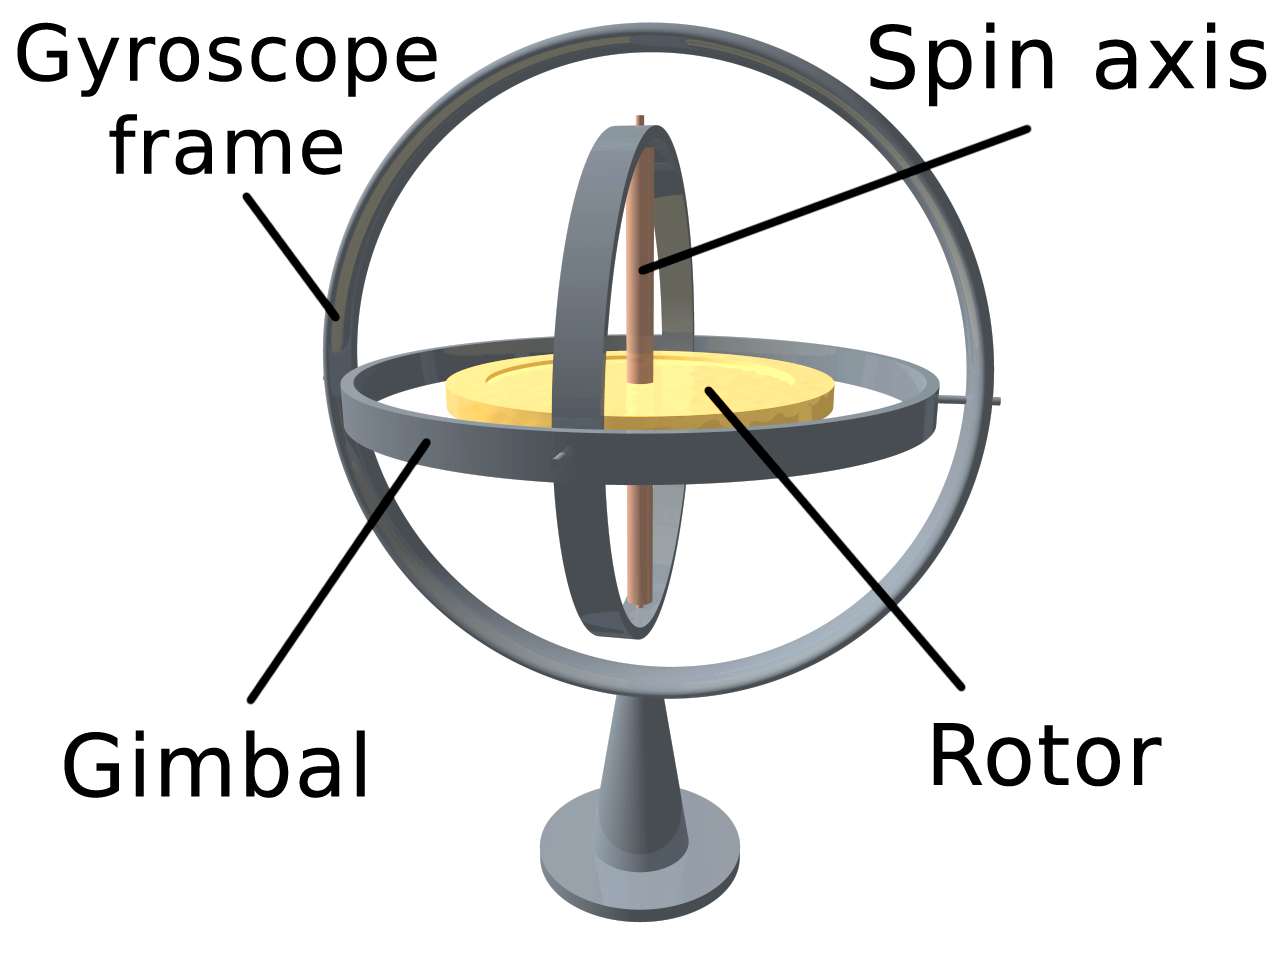
\includegraphics[width=3in]{Image Gyroscope.png}
\end{center}
\tiny{\textbf{Fig. 14.} Gyroscope - Wikipedia. https://en.wikipedia.org/wiki/Gyroscope. Accessed 13 Apr. 2022.}
\end{frame}

\begin{frame}{Accelerometers}
\begin{center}
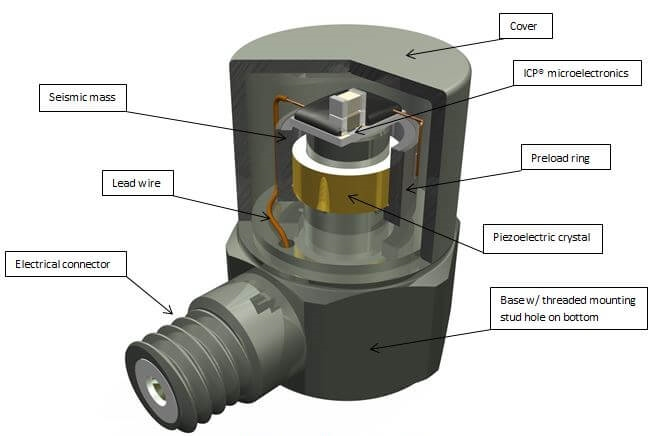
\includegraphics[width=3.4in]{Image Accelerometer.jpg}
\end{center}
\tiny{\textbf{Fig. 15.} Introduction to Piezoelectric Accelerometers. https://www.pcb.com/resources/technical-information/introduction-to-accelerometers. Accessed 13 Apr. 2022.}
\end{frame}

\begin{frame}{Magnetometers}
\begin{center}
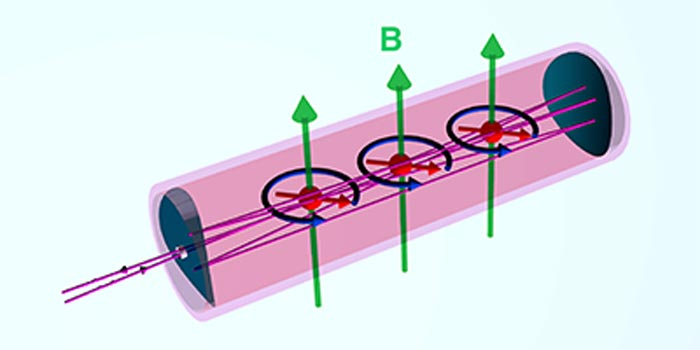
\includegraphics[width=3.8in]{Image Magnetometer.jpg}
\end{center}
\tiny{\textbf{Fig. 16.} “Atomic Magnetometer Is Most Sensitive Yet.” Physics World, 24 Apr. 2013, https://physicsworld.com/a/atomic-magnetometer-is-most-sensitive-yet/.}
\end{frame}

\begin{frame}{My future in Virtual Reality}
Programming my own Virtual Reality in Unity and C\# this coming Fall for Senior Thesis
\vskip .2in
Virtual Reality Video Game Programming
\end{frame}

\begin{frame}{References}
\setbeamertemplate{bibliography item}{\insertbiblabel}
\begin{thebibliography}{9}

\bibitem{A} Grasnick, Armin. Basics of Virtual Reality: From the Discovery of Perspective to VR Glasses. Springer Berlin Heidelberg, 2021.

\bibitem{B} This Is the Engineering Behind How VR Headsets Work. 9 May 2020, https://interestingengineering.com/vr-headsets-work-through-a-combination-of-different-tracking-technologies.

\bibitem{C} Verma, Jitendra Kumar, and Sudip Paul, editors. Advances in Augmented Reality and Virtual Reality. Springer Singapore, 2022.
\end{thebibliography}
\end{frame}
\end{document}